% Document preamble
\documentclass{article}
\usepackage{lipsum}
\usepackage{graphicx}
\usepackage[table]{xcolor}
\usepackage{titlesec}
\usepackage{soul}
\usepackage{listings}
\usepackage{caption}

% Global settings for listings
\lstset{
    basicstyle=\ttfamily\small,   % Font size and style for code
    frame=single,                 % Frame around code
    breaklines=true,              % Enable line breaks
    captionpos=b,                 % Position of caption
    numbers=left,                 % Line numbers on the left
    numberstyle=\tiny\color{gray} % Style for line numbers
}

% HTML settings
\lstdefinelanguage{HTML}{
    language=HTML,
    sensitive=true,
    morecomment=[s]{<!--}{-->},       % HTML comment style
    morestring=[b]",                  % String style
    tagstyle=\color{purple},          % Tag style
    keywordstyle=\color{blue},        % Keyword style
    commentstyle=\color{green},       % Comment style
    stringstyle=\color{red},          % String style
    morekeywords={<!DOCTYPE,html,head,title,body,div,span,script,style,h1,h2,h3,p,a,img,ul,li,table,tr,td,th}, % HTML tags
}

% CSS settings
\lstdefinelanguage{CSS}{
    language=CSS,
    sensitive=true,
    morecomment=[l]{//},              % Comment style
    morecomment=[s]{/*}{*/},          % Block comment style
    morestring=[b]",                  % String style
    keywordstyle=\color{blue},        % Property names
    commentstyle=\color{green},       % Comment style
    stringstyle=\color{red},          % String style
    morekeywords={color,background,font-size,font-family,border,margin,padding,width,height,display,position,top,bottom,left,right,float,clear,overflow}, % CSS properties
}

\usepackage{amsmath}
\usepackage{xcolor}
\usepackage{circuitikz}
\usepackage{tikz}
\usetikzlibrary{positioning, shapes.geometric, arrows}
\usepackage{float}
\usepackage{url}
\usepackage{pgfplots,pgfplotstable}
\pgfplotsset{compat=1.18}
\date{\today}

%Packages for costum tables 
\usepackage{booktabs, multirow}
\usepackage{changepage,threeparttable} 

% Set the document layout 
\usepackage{multicol}
\usepackage{geometry}
\geometry{margin=1.5cm}

% Set the authors and affiliation
\usepackage{authblk}
\author{Kasandikromo Guillian}
\author{Karg Timothy}
\author{Uraicia Sewpersad}
\affil{Vanguard Community College - Department of Engineering}

% Modify the authors and affilition text 
\renewcommand\Authfont{\bfseries\fontsize{9}{14}\selectfont}
\renewcommand\Affilfont{\fontsize{12}{14}\selectfont}

% Set the header of the document
\usepackage{fancyhdr}
\pagestyle{fancy}
\fancyhf{}
\fancyhead[L]{\fontsize{8}{12}\selectfont Vanguard Community College}
\fancyhead[C]{\fontsize{8}{12}\selectfont \date{\today}}
\fancyhead[R]{\fontsize{8}{12}\selectfont Page \thepage}

% Modify the header lenght, width and position
\newlength\FHleft
\newlength\FHright
\setlength\FHleft{1cm}
\setlength\FHright{0cm}
\setlength{\headheight}{25pt}

% Set the separation lenght of the columns
\setlength{\columnsep}{1cm}

% Set the titel of the document
\title{\Large \bfseries 
    Monitoring Energy Consumption using Arduino}

% Redefine the section numbering format
\renewcommand{\thesection}{\Roman{section}.}
\renewcommand{\thesubsection}{\roman{subsection}.}
\titlespacing*{\section}{0pt}{1cm}{0.5cm}
\titlespacing*{\subsection}{0pt}{0.5cm}{2pt}
\titleformat{\section}
  {\bfseries\large\centering}{\thesection}{1em}{}
\titleformat{\subsection}
  {\normalsize\centering\itshape}{\thesubsection}{1em}{}

\begin{document}
    \begin{multicols}{2}
        \maketitle
        \thispagestyle{fancy}
       \begin{abstract}
        \setlength{\baselineskip}{1.2\baselineskip} % Increase line spacing
        \noindent 
        \makebox[\linewidth]{
            \begin{minipage}{0.48\textwidth}
            This project explains how to set up an Arduino-based system to measure and monitor energy use, making the data accessible in real-time through cloud storage and a web app. As energy optimization becomes more important, this setup provides accurate and easily accessible energy data to help users make informed decisions.

The system uses an Arduino microcontroller with a YHDC Current Transformer SCT-013-000 sensor to measure current. The Arduino converts this data into energy consumption readings in kilowatt-hours (kWh) after first calculating power (watts) and then energy (watt-seconds). Every 10 seconds, this data is sent to a cloud-based PostgreSQL database via a Python script, which connects to the Arduino’s serial output.

To make the data easy to view and analyze, a web app built with Flask and Dash lets users filter data by month or day to explore detailed energy usage patterns. The app also updates automatically, so the latest measurements are always available. With data stored in the cloud, users can monitor energy use from anywhere, helping them identify opportunities to save energy.

Overall, this system combines Arduino's compatibility with various sensors and the cloud’s accessibility, creating a reliable and scalable solution for tracking energy usage in real time.

            \end{minipage}}
        \end{abstract}
    
        % Set sections and bibliography
        \section{Introduction}

This project aims to develop and deploy an Energy Monitor system, designed to provide real-time energy consumption data for a residential setting. The core component of the system is an Arduino-based microcontroller, responsible for collecting and processing energy consumption data from various sensors. This data is then transmitted to a web server, allowing for remote monitoring and analysis. 

The web application, built using Python and Flask, provides a user-friendly interface to visualize energy consumption patterns, identify potential areas for energy savings, and generate insightful reports. This project leverages the power of open-source technologies to create a cost-effective and customizable solution for energy monitoring.

Key Features:
\begin{itemize}
    \item Real-time monitoring: The system provides up-to-date energy consumption data.
    \item Remote access: Users can access and analyze data from anywhere with an internet connection.
    \item Data visualization: The web application offers various visualization tools for easy data interpretation.
    \item Energy efficiency insights: The system helps identify areas for energy savings and optimization.
\end{itemize}

This document will detail the system's architecture, hardware implementation, software development, and deployment process. It will also include a comprehensive evaluation of the system's performance and potential future enhancements.
        \section{Materials}
\lipsum[1-1]
\subsection{Arduino Micro-controller}

\begin{itemize}
    \item Microcontroller: The heart of the project. It processes the data received from sensors, performs calculations, and controls other components.
    \item Digital and Analog Pins: These pins are used to connect sensors and actuators. Digital pins provide high or low signals, while analog pins can read varying voltage levels.
    \item Power Supply: The board can be powered by a USB cable or an external power supply.
    \item Serial Communication: The board can communicate with a computer or other devices using a serial connection.
\end{itemize} 

\subsection{YHDC Current Transformer SCT-013-000}
    \begin{minipage}{\linewidth}
\begin{figure}[H]
\centering
    \begin{circuitikz}
        \tikzstyle{every node}=[font=\small]
        \draw [](1.25,11.5) to[short] (3,11.5);
        \draw [](1.25,11.5) to[short, -o] (0.75,11.5);
        \draw [->, >=Stealth] (1.75,11.5) -- (2,11.5);
        
        \draw [](3,11.5) to[short] (3,10.75);
        \draw [](3,11) to[short] (3,10.5);
        \draw (3,10.5) to[L ] (5,10.5);
        
        \draw [](5,10.5) to[short] (5,11.5);
        \draw [](5,11.5) to[short] (6.5,11.5);
        \draw [](6.5,11.5) to[short, -o] (7,11.5) ;
        \draw [->, >=Stealth] (6,11.5) -- (6.25,11.5);
        \draw (2.75,9.5) to[L ] (5.25,9.5);
        
        \draw[] (5.25,9.5) to[short] (5,9.5);
        
        \draw[] (5,9.5) to[short] (4.75,9.5);
        \draw [, dashed] (2.75,11) rectangle  (5.25,9.25);
        \draw [](2.75,9.25) to[short] (2.75,8.75);
        \draw [](2.75,8.75) to[short] (2.75,8.25);
        
        \draw [](5.25,9.25) to[short] (5.25,8.25);
        \draw[] (5.25,8.25) to[short] (4.5,8.25);
        \node at (4.5,8.25) [circ] {};
        \draw [](4.5,8.25) to[short] (4.5,6.25);
        \node at (2.75,8.25) [circ] {};
        
        \draw [](2.75,8.25) to[short] (2.75,5.75);
        \draw (2.25,7.25) to[C] (1.5,7.25);
        \node at (2.75,7.25) [circ] {};
        \draw (2.25,7.25) to[C] (1,7.25);
        \draw [](2.75,5.75) to[short] (2.75,5.5);
        \draw [](2.75,5.5) to[short] (2.75,5.25);
        \node at (2.75,5.25) [circ] {};
        \draw (2.75,5.25) to[R] (4.75,5.25);
        \draw (2.25,5.25) to[R] (1,5.25);
        \draw [](2.25,5.25) to[short] (2.75,5.25);
        \draw [](2.25,7.25) to[short] (2.75,7.25);
        \draw[] (1,5.25) to[short] (0.75,5.25);
        \draw[] (1,7.25) to[short] (0.75,7.25);
        \draw[] (0.75,5.25) to[short] (0.5,5.25);
        \draw[] (0.75,7.25) to[short] (0.5,7.25);
        \node at (0.5,7.25) [circ] {};
        \node at (0.5,5.25) [circ] {};
        \draw [](0.5,5.25) to[short] (0.5,7.25);
        \draw [](0.5,7.25) to[short] (0.5,8.25);
        \draw [](0.5,5.25) to[short] (0.5,4);
        \draw [](2.75,5.25) to[short] (2.75,4.25);
        \draw [](2.75,4.25) to[short] (2.75,4);
        \draw [](4.5,6.25) to[short] (4.5,4);
        \draw [](4.5,5.25) to[short] (5,5.25);
        \draw [](4.75,5.25) to[short] (5.5,5.25);
        \draw [](5.5,5.25) to[short] (5.5,4);
        \node [font=\small] at (1.75,11.75) {Heavy line current};
        \node [font=\small] at (6.75,10) {Current transformer};
        \node [font=\small] at (4,9) {Secondary};
        \node [font=\small] at (4,11.25) {Primary};
        \node [font=\small] at (6,11.75) {To load};
        \node [font=\small] at (1.75,8) {C1 10$\mu$F};
        \node [font=\small] at (1.75,5.75) {R1 10k$\Omega$};
        \node [font=\small] at (3.75,5.75) {R2 10k$\Omega$};
        \draw [](2.75,8.25) to[short] (4.5,8.25);
        \node [font=\small] at (6.25,8.75) {C.T Output};
        \node [font=\small, rotate around={270:(0,0)}] at (0.25,4.5) {Arduino GND};
        \node [font=\small, rotate around={270:(0,0)}] at (4.25,4) {Arduino input};
        \node [font=\small, rotate around={270:(0,0)}] at (5.75,4.5) {Arduino 5V DC};
        \node [font=\small, rotate around={270:(0,0)}] at (2.5,4.5) {Mid-point};
        \draw [](5.5,3.75) to[short, o-] (5.5,4) ;
        \draw [](0.5,3.75) to[short, o-] (0.5,4) ;
        \draw [](4.5,3.75) to[short, o-] (4.5,4) ;
        \draw [](2.75,4) to[short] (2.75,3.75);
    \end{circuitikz}
    \caption{Current transformer circuit with Arduino}
    \label{fig:CT - Sensor}
\end{figure}
\vspace{2pt}
\end{minipage}
\begin{itemize}
    \item  Non-invasive Measurement: It measures the current flowing through a wire without physically breaking the circuit.
    \item Magnetic Induction: It works based on the principle of electromagnetic induction.
    \item Output Signal: It produces a small AC voltage proportional to the current flowing through the wire.
    \item Safety: It allows for safe measurement of high currents without the risk of electric shock.
\end{itemize}

\subsection{Liquid Crystal Display}
\begin{itemize}
    \item Display: It displays information like voltage, current, power consumption, and other relevant data.
    \item Backlight: It provides illumination for better visibility.
    \item Interface: It connects to the Arduino board through digital pins to receive and display data. 
    \item Types: There are various types of LCDs, including character LCDs and graphic LCDs. \cite{OpenEnergyMonitor}
\end{itemize} 

\subsection{ Other Potential Components:}
\begin{itemize}
    \item Voltage Sensor: Measures the voltage entering the circuit.
    \item Temperature Sensor: Monitors the temperature of the system or environment.
    \item Power Supply: Provides the necessary power for the Arduino and other components.
    \item Resistors: Used to limit current and divide voltage.
    \item Capacitors: Used to filter noise and store energy.
\end{itemize}
        \section{System Design}
\label{sec:system_design}

\noindent The energy monitoring system consists of three main components:
the Arduino microcontroller, the YHDC Current Transformer (CT) SCT-013-000 sensor, and a cloud-based PostgreSQL database accessible through a web application. Each component plays a vital role in capturing, processing, storing, and displaying energy consumption data in real-time.

\subsection{Hardware Components}
\noindent The system's hardware includes:
\begin{itemize}
    \item \textbf{Arduino Microcontroller:} The Arduino serves as the primary data collection unit, converting analog signals from sensors to digital data for processing. It calculates the instantaneous power and energy usage based on current measurements from the CT sensor.
    \item \textbf{YHDC SCT-013-000 Current Transformer Sensor:} This non-invasive sensor measures the AC current flowing through a wire. It generates an analog signal proportional to the current, which is read by the Arduino's analog input.
    \item \textbf{AC-to-AC Power Adapter:} To measure AC voltage, an AC-to-AC adapter is used. This adapter steps down the AC voltage to a safe level compatible with the Arduino's analog input, allowing it to monitor real-world voltage values accurately.
\end{itemize}

\subsection{Software Components}
\noindent The software components of the system include:
\begin{itemize}
    \item \textbf{Data Processing on Arduino:} The Arduino processes signals from the CT sensor and calculates power by combining current and voltage values. The calculated energy data is sent to a local SQLite database, which is later synced with a cloud database.
    \item \textbf{Python Data Transfer Script:} A Python script interfaces with the Arduino's serial monitor and transfers the processed data to a cloud-based PostgreSQL database at intervals of 10 seconds.
    \item \textbf{Flask Web Application:} A Flask-based application with Dash visualizes the data, allowing users to filter by month and day to observe consumption trends. This user interface provides an accessible and flexible way to monitor energy usage over time.
\end{itemize}

\subsection{Data Flow and Operation}
\begin{minipage}{\linewidth}
    \centering
    \begin{tikzpicture}[
        % Define styles for the components
        block/.style={rectangle, draw, text centered, rounded corners, minimum height=2em, minimum width=3cm, fill=gray!10},
        arrow/.style={thick,->,>=stealth},
        sensor/.style={diamond, draw, text centered, minimum height=2em, minimum width=2em, fill=blue!10},
        storage/.style={cylinder, draw, shape border rotate=90, aspect=0.25, minimum height=2cm, minimum width=1cm, fill=green!20}
    ]
    
    % Define nodes
    \node[block] (power) {Power Source};
    \node[sensor, below=of power] (sensor) {CT Sensor};
    \node[block, below=of sensor] (arduino) {Arduino Microcontroller};
    \node[storage, below=of arduino] (database) {Cloud Database};

    % Draw arrows
    \draw[arrow] (power) -- (sensor) node[midway, right] {AC Current};
    \draw[arrow] (sensor) -- (arduino) node[midway, right] {Analog Signal};
    \draw[arrow] (arduino) -- (database) node[midway, right] {Energy Data (kWh)};

    % Add annotations
    \node[below=0.3cm of database, align=center] {Data stored in PostgreSQL database \\ accessible by web app};
    \end{tikzpicture}
    \captionof{figure}{\small \indent Process Flow Diagram of the Energy Monitoring System}
    \vspace{0.5cm}
    \label{fig:PFD}
\end{minipage}
\noindent The system operates as follows:
\begin{enumerate}
    \item The Arduino reads analog signals from the CT sensor and the AC-to-AC adapter.
    \item It processes these signals, calculates energy consumption in watt-seconds (later converted to kWh), and sends the data to the Python script.
    \item The Python script logs the data in a local SQLite database, which then syncs to a PostgreSQL cloud database every 10 seconds.
    \item The web app fetches the latest data from the cloud database, displaying it with interactive filters for user analysis.
\end{enumerate}

\noindent This modular design, combining hardware and software elements, enables real-time, remote monitoring of energy usage.

        \section{Measuring AC Voltage with an AC to AC power adapter}
\lipsum[1-2]
\begin{minipage}{\linewidth}
\begin{table}[H]
    \centering
    \caption{AC-AC Voltage Transformator Data }
    \label{tab:voltage transformator }
    \small
    \begin{tabular*}{\linewidth}{@{\extracolsep{\fill}}ccc}
    \textbf{V (input) (V)} &\textbf{I (mA)} &\textbf{V(output) (mV)} \\\midrule
    10 &0.59 &3.6 \\
    20 &1.15 &8.6 \\
    30 &1.7 &12.8 \\
    40 &2.25 &16.9 \\
    50 &2.8 &21.2 \\
    60 &3.4 &25.3 \\
    70 &3.96 &29.6 \\
    80 &4.52 &33.6 \\
    90 &5 &38 \\
    100 &5.67 &42.2 \\
    110 &6.21 &46.4 \\
    120 &6.77 &51 \\
    130 &7.38 &55.2 \\
    140 &7.9 &59.1 \\
    \bottomrule
    \end{tabular*}
\end{table}
\begin{tikzpicture}
    \begin{axis}[
    title={AC-AC Voltage Transformator Input vs. Output},
    ticklabel style={font=\scriptsize},
    xlabel={V (input) (V)},
    ylabel={V(output) (mV)},
    xmin=0, xmax=150,
    ymin=0, ymax=60,
    xtick={0,10,20,30,40,50,60,70,80,90,100,110,120,130,140},
    ytick={0,10,20,30,40,50,60},
    legend pos=north west,
    ymajorgrids=true,
    grid style=dashed,
    xmajorgrids=false
]
    \addplot[
        color=red!80,
        mark=circle,
    ]
    coordinates {
        (10,3.6)(20,8.6)(30,12.8)(40,16.9)(50,21.2)(60,25.3)(70,29.6)(80,33.6)(90,38)(100,42.2)(110,46.4)(120,51)(130,55.2)(140,59.1)
    };
    \addlegendentry{V(output) (mV)}
    \label{fig:V in-out}
    \end{axis}
\end{tikzpicture}
\end{minipage}

        \end{multicols}

        %\section{Overview of the Application}

% Preset code colors for python 
\lstset{
    language=Python,             % Language of the code
    basicstyle=\ttfamily\small,  % Basic font style
    keywordstyle=\color{blue},   % Style for keywords
    commentstyle=\color{green},  % Style for comments
    stringstyle=\color{red},     % Style for strings
    frame=single,                % Draw a frame around the code
    breaklines=true,             % Allow line breaks within code
    captionpos=b,                % Set the caption position to bottom
    numbers=left,                % Add line numbers on the left
    numberstyle=\tiny\color{gray}, % Style for line numbers
}

The application consists of the following components:
\begin{itemize}
    \item \textbf{Backend (app.py):} Built with Flask, it fetches data from a PostgreSQL database, processes it, and serves it to the front-end.
    \item \textbf{Frontend (index.html):} A responsive HTML page styled with CSS, allowing users to select filters and view energy data in a Plotly graph.
    \item \textbf{CSS (style.css):} Defines styles for the HTML elements to make the dashboard user-friendly and visually appealing.
\end{itemize}

\section{Backend Code (app.py)}

The main backend code in \texttt{app.py} initializes the Flask app, loads environment variables, connects to the PostgreSQL database, and defines routes for data retrieval and front-end rendering.

\subsection{Code Listing}
Below is the \texttt{app.py} code, with comments explaining each section.

\begin{lstlisting}[language=Python, caption=app.py, frame=single]
# Import necessary libraries
from flask import Flask, render_template, jsonify, request
import pandas as pd
import plotly.graph_objects as go
from dotenv import load_dotenv
import os
import psycopg2
from psycopg2 import OperationalError

# Initialize Flask application
app = Flask(__name__)

# Load environment variables from the .env file for secure configuration
load_dotenv()

# Get the database connection URL from environment variables
DATABASE_URL = os.getenv("DATABASE_URL")

# Define function to fetch and process data from the PostgreSQL database
def get_data(tab, group_by=None, selected_month=None, selected_day=None):
    try:
        # Connect to the database
        conn = psycopg2.connect(DATABASE_URL)
        query = "SELECT date, irms, energy_usage, kwh FROM energydata"
        df = pd.read_sql_query(query, conn)  # Read data into a DataFrame
        conn.close()  # Close the connection after fetching data
    except OperationalError as e:
        print("Error connecting to the database:", e)
        return pd.DataFrame()  # Return empty DataFrame if connection fails

    # Process date and extract date components for filtering
    df['date'] = pd.to_datetime(df['date'], format='%Y-%m-%d %H:%M:%S', errors='coerce')
    df['year'] = df['date'].dt.year
    df['month'] = df['date'].dt.month_name()
    df['day'] = df['date'].dt.day
    df['hour'] = df['date'].dt.hour
    df = df.sort_values(by='date')  # Sort data by date for plotting

    # Apply filters based on selected month and day
    if selected_month:
        df = df[df['month'] == selected_month]
        df = df.sort_values(by=['day', 'date'])
    if selected_day:
        df = df[df['day'] == int(selected_day)]
        df = df.sort_values(by=['hour', 'date'])

    return df  # Return filtered data

# Define the main route for the application
@app.route('/')
def index():
    # Retrieve user-selected month, day, and metric type from the URL parameters
    selected_month = request.args.get('month')
    selected_day = request.args.get('day')
    selected_tab = request.args.get('tab', 'irms')  # Default to 'irms' tab if none selected

    # Fetch and filter data based on user selections
    df = get_data(tab=selected_tab, selected_month=selected_month, selected_day=selected_day)

    # Create Plotly figure based on the selected tab (irms, energy_usage, or kWh)
    fig = go.Figure()
    if selected_tab == 'irms':
        fig.add_trace(go.Scatter(x=df['date'], y=df['irms'], mode='lines', name='Irms'))
        fig.update_layout(title="Current (Irms)", xaxis_title="Date", yaxis_title="Current (A)")
    elif selected_tab == 'energy_usage':
        fig.add_trace(go.Scatter(x=df['date'], y=df['energy_usage'], mode='lines', name='Energy Usage'))
        fig.update_layout(title="Energy Usage (Ws)", xaxis_title="Date", yaxis_title="Energy (Ws)")
    else:
        fig.add_trace(go.Scatter(x=df['date'], y=df['kwh'], mode='lines', name='kWh'))
        fig.update_layout(title="Energy Consumption (kWh)", xaxis_title="Date", yaxis_title="kWh")

    # Convert Plotly figure to HTML to embed in the front-end
    graph_html = fig.to_html(full_html=False)

    # Prepare month and day options for dropdowns in the front-end
    month_options = [{'value': month, 'label': month} for month in df['month'].unique()]
    day_options = df['day'].unique().tolist()

    # Render the front-end template with graph and dropdown options
    return render_template('index.html', 
                           graph_html=graph_html,
                           selected_month=selected_month, 
                           selected_day=selected_day,
                           selected_tab=selected_tab,
                           month_options=month_options,
                           day_options=day_options)

# Route to fetch day options dynamically when a month is selected
@app.route('/days', methods=['GET'])
def get_days():
    selected_month = request.args.get('month')
    df = get_data(tab='irms', selected_month=selected_month)
    days = df['day'].unique().tolist()
    return jsonify(days)

# Run the Flask app
if __name__ == '__main__':
    app.run(debug=True)
\end{lstlisting}

\section{Frontend Code (index.html)}

The HTML template for the dashboard displays dropdown menus for filtering by month and day, tab navigation, and the Plotly graph.

\subsection{Code Listing}
Below is the \texttt{index.html} code with added comments.

\begin{lstlisting}[language=HTML, caption=index.html, frame=single]
<!DOCTYPE html>
<html lang="en">
<head>
    <!-- Meta tags and imports for responsive design -->
</head>
<body>
    <div class="container">
        <header>
            <h1>Energy Data Dashboard</h1>
        </header>

        <!-- Dropdown Filters for selecting Month and Day -->
        <div class="dropdowns">
            <div class="dropdown-container">
                <label for="month-dropdown">Select Month</label>
                <select id="month-dropdown">
                    <option value="">-- Select Month --</option>
                    
                        <!-- Pre-select the chosen month in the dropdown -->
                        <option value="{{ month['value'] }}" selected>{{ month['label'] }}</option>
                    
                </select>
            </div>
            <div class="dropdown-container">
                <label for="day-dropdown">Select Day</label>
                <select id="day-dropdown" disabled>
                    <option value="">-- Select Day --</option>
                    
                        
                            <option value="{{ day }}" selected>Day {{ day }}</option>
                        
                    
                </select>
            </div>
        </div>

        <!-- Tabs for selecting the data type (Irms, Energy Usage, or kWh) -->
        <div class="tabs-and-reset">
            <!-- Tab elements go here -->
        </div>

        <!-- Container for the Plotly graph -->
        <div id="plotly-graph" class="graph-container">
            {{ graph_html | safe }}
        </div>

        <footer>
            <p>© 2024 Energy Data Dashboard. All rights reserved.</p>
        </footer>
    </div>
</body>
</html>
%\end{lstlisting}

\section{CSS Code (style.css)}

The CSS file customizes the appearance of the dashboard, including layout, colors, and responsive adjustments for different screen sizes.

\subsection{Code Listing}
Below is the \texttt{style.css} code with added comments.

\begin{lstlisting}[language=CSS, caption=style.css, frame=single]
/* General Reset and Global Styles */
* {
    margin: 0;
    padding: 0;
    box-sizing: border-box;
}

body {
    font-family: 'Poppins', sans-serif;
    background: linear-gradient(135deg, #e2f095 0%, #3498db 100%);
    color: #333;
    line-height: 1.6;
    padding: 20px;
}

/* Container Styling */
.container {
    max-width: 1200px;
    margin: 0 auto;
    padding: 40px;
    background-color: #ffffff;
    border-radius: 15px;
    box-shadow: 0 12px 30px rgba(0, 0, 0, 0.1);
}

/* Header Styling */
header {
    text-align: center;
    margin-bottom: 40px;
}

h1 {
    color: #34495e;
    font-size: 3.5em;
    font-weight: 600;
    text-transform: uppercase;
    letter-spacing: 2px;
}

/* Dropdown Styling */
.dropdowns {
    display: flex;
    justify-content: space-between;
    gap: 20px;
    margin-bottom: 30px;
    flex-wrap: wrap; /* Allow wrapping on small screens */
}

.dropdown-container {
    flex: 1;
    min-width: 200px;  /* Ensures it doesn't get too small on mobile */
}

select {
    padding: 12px 18px;
    font-size: 1.1em;
    border-radius: 8px;
    border: 1px solid #ddd;
    width: 100%;
    transition: all 0.3s ease;
    background-color: #fafafa;
    color: #2c3e50;
}

select:focus {
    border-color: #3498db;
    background-color: #fff;
    outline: none;
}

select:hover {
    border-color: #3498db;
    cursor: pointer;
}

/* Tab Styling */
.tabs {
    margin-bottom: 30px;
}

.tab-titles {
    list-style: none;
    display: flex;
    justify-content: center;
    gap: 20px;
    padding: 0;
}

.tab-titles li {
    font-size: 1.2em;
    cursor: pointer;
}

.tab-titles a {
    text-decoration: none;
    color: #2c3e50;
    padding: 10px 20px;
    border-radius: 8px;
    background-color: #f5f5f5;
    transition: all 0.3s ease;
}

.tab-titles a:hover,
.tab-titles li.active a {
    background-color: #3498db;
    color: white;
}

/* Graph Container Styling */
.graph-container {
    width: 100%;
    height: 600px;
    background-color: #ffffff;
    border-radius: 10px;
    box-shadow: 0 4px 15px rgba(0, 0, 0, 0.1);
}

/* Footer Styling */
footer {
    text-align: center;
    margin-top: 50px;
    font-size: 1em;
    color: #7f8c8d;
}

/* Tabs and Reset Container */
.tabs-and-reset {
    display: flex;
    justify-content: space-between;
    align-items: center;
    gap: 20px;
    margin-bottom: 20px;
}

#reset-button {
    background-color: #e74c3c;
    color: white;
    border: none;
    padding: 12px 20px;
    font-size: 1.2em;
    cursor: pointer;
    border-radius: 8px;
    display: inline-flex;
    align-items: center;
    gap: 8px;
}

#reset-button i {
    font-size: 1.4em;
}

#reset-button:hover {
    background-color: #c0392b;
}

/* Responsive Styles */
@media (max-width: 768px) {
    .dropdowns {
        flex-direction: column;
        gap: 10px;
    }

    .tab-titles {
        flex-direction: column;
        gap: 10px;
    }

    .tabs-and-reset {
        flex-direction: column;
        align-items: flex-start;
        gap: 10px;
    }

    #reset-button {
        width: 100%;
        text-align: center;
    }
} 
\end{lstlisting} 
        \bibliographystyle{plain}
        \bibliography{Reference}
\end{document}